\chapter{基于分层级联音乐对齐的三维数字人舞蹈生成}
\section{本章引言}
舞蹈作为人类文明中重要的艺术表达形式与文化遗产，能够以非语言的方式传达情绪与叙事内容，其表现依赖于身体运动、手部姿态以及面部表情等多维度信息的协同~\cite{fink2021evolution, kico2018digitization}。近年来，随着电子游戏、虚拟现实与数字演出等数字娱乐产业的快速发展，面向真实感与表现力的三维舞蹈动画需求持续增长。然而，传统舞蹈资产获取通常依赖专业舞者与昂贵的动作捕捉系统，制作过程劳动密集、周期长且成本高，显著制约了舞蹈内容的规模化生产与应用落地。因此，如何基于音乐自动生成高质量舞蹈序列成为计算机图形学与多模态生成领域的重要研究问题。

早期方法主要基于运动图（motion graph）~\cite{arikan2002interactive, kim2003rhythmic, shiratori2006dancing, kim2006making, tang2018dance}进行动作片段重组，能够在局部层面保持运动连续性与物理合理性，但难以显式建模音乐与舞蹈之间的内在对应关系。随后，FACT~\cite{li2021ai}、EDGE~\cite{tseng2023edge}等学习式方法采用滑动窗口或局部片段学习策略提升局部动作质量，但往往忽略编舞层面的全局结构一致性。近期，Bailando~\cite{siyao2022bailando}引入 VQ-VAE~\cite{van2017neural}并结合强化学习以增强节奏对齐能力，但其训练流程复杂、泛化能力受限。FineNet~\cite{li2023finedance}进一步同时建模身体与手部动作，但仍无法生成与动作相匹配的面部表情，导致生成结果在情绪表达层面不完整。

总体而言，尽管现有研究取得一定进展，生成与音乐同步且整体协调的高质量舞蹈序列仍面临挑战，主要体现在以下三个方面。第一，数据层面仍存在不足：现有音乐-舞蹈数据集要么缺失表演关键要素，要么受限于采集精度与质量。例如，AIST++\cite{li2021ai}主要提供与音乐对应的身体动作数据；FineDance\cite{li2023finedance}与 Choreomaster~\cite{chen2021choreomaster}虽包含更细粒度的手指运动信息，但仍缺少面部表情这一关键情绪载体。此外，多数数据集基于视频姿态估计得到骨架序列，难以避免估计误差与噪声，从而影响训练与评测的可靠性。第二，建模层面存在能力瓶颈：现有方法对身体、手部与面部之间复杂的层级依赖关系刻画不足，难以生成三者在空间与时间上高度协调的整体动作。第三，跨模态对齐仍不充分：音乐与舞蹈之间缺乏精细的对齐机制，导致节奏与情绪等维度的同步效果不佳。

针对上述问题，本文从数据集与方法两方面提出系统性解决方案。首先本章提出了高表现力的全身舞蹈动作数据集SoulDance，其采用了专业的全身动作捕捉系统对舞蹈动作进行采集，在时间与空间维度上实现了身体、手部与面部的精准协同，以及舞蹈和音乐之间的精密对齐。

在SoulDance数据集基础上，本章进一步提出整体舞蹈生成框架 SoulNet，其核心由三部分组成，用于同时解决动作协调与跨模态对齐问题。第一，为提升身体、手部与面部的协同生成能力，本文提出层次化残差量化编码（Hierarchical Residual Vector Quantization），它在残差向量量化（RVQ）~\cite{barnes1996advances,huijben2024residual}的基础上构建多层编码结构，并通过“身体-手部-面部”链式设计显式建模三者之间的空间关系与层级依赖。第二，为实现音乐条件下的序列生成与同步，本文设计音乐-舞蹈对齐生成模块\textit{MAGM}，采用基于 Transformer 的生成架构，将层级化舞蹈单元组合为全局连贯的舞蹈序列，同时保持与音乐的节奏一致性。第三，本文引入预训练的音乐动作检索模块（MMR），利用大规模公开音乐-舞蹈数据学习对齐先验，并以检索得到的先验作为生成过程的对齐引导，从而进一步提升跨模态一致性。与此同时，为更全面地评估音乐-舞蹈对齐效果，本文提出两项新指标：情感对齐分数，用于量化面部表情与音乐情绪基调的一致性；音乐对齐分数，用于细粒度评估音乐节奏与舞蹈动作之间的同步程度。相较于现有主要依赖粗粒度风格标签的指标（如 Genre-Matching Score~\cite{li2023finedance}），上述指标能够提供更精确、更全面的评测。总体来说，本章的主要贡献总结如下：
\begin{itemize}
    \item 提出舞蹈动作的数据集 SoulDance：一个新的高质量强对齐的舞蹈动作数据集，覆盖身体动作、手部姿态与面部表情，并在规模与完整性方面达到目前同类数据集的领先水平。
    \item 提出舞蹈动作生成网络 SoulNet：首先，提出HRVQ实现对动作的精细表征提升舞蹈动作精细度以及动作间协调性，然后利用音乐-舞蹈对齐先验来实现整体舞蹈协同建模的生成框架，在节奏与情绪维度上提升音乐与舞蹈的一致性。
    \item 提出新的评价指标：情感对齐分数与音乐对齐分数两项指标，用于更精确评估面部与身体动作与音乐之间的对齐程度；并在多个数据集上的实验结果表明，本文方法在上述指标及公开基准上均取得了优异性能。
\end{itemize}



% \section{拟解决的关键问题}
% 围绕高表现力三维数字人舞蹈动作生成，本课题主要聚焦四个关键问题：第一，在尽量低的数据与计算成本下实现数字人外观的快速定制和编辑，涵盖面部五官与肤质细节、发型与发色、服装款式与材质纹理、配饰及风格化元素等；同时需保证在不同姿态与镜头视角下外观一致，为后续动作驱动与多视角渲染提供稳定可靠的角色基础。第二，构建全身协调的舞蹈动作数据集：既要确保动作数据质量高、噪声与伪影可控，又要覆盖多风格、多难度的舞蹈类型与动作分布，并配套准确的音乐、节拍与时序标注，以支撑端到端训练与客观评测。第三，设计全身协调的动作编码与建模方式：对身体动作、手部姿势与面部表情进行统一表征与联合建模，刻画不同部位之间的时空依赖与互相约束，捕捉“手—身—脸”协同的运动规律，从而提升生成动作的自然性与感染力。第四，实现音乐对齐的舞蹈动作生成机制：在生成过程中显式建模音乐的节奏结构与情绪线索，使舞蹈动作在节拍、重音与段落结构上与音乐特征一致，并在动作强度、风格表达与情绪传递上形成匹配，从而进一步提升整体舞蹈的协调性与表现力。

% \subsection{高效的三维数字人外观编辑}
% 在扩散式文本引导生成/编辑框架下，实现无需或少训练、低计算开销的个性化外观编辑，并兼顾局部可控性与身份一致性。现有T2I~\cite{saharia2022photorealistic,ramesh2022hierarchical}扩散模型虽能在大规模图文数据上生成高质量、多样化图像，并已拓展到图像编辑与个性化等任务，但多数编辑方法仍依赖手工掩码完成局部编辑，且在修改语义属性时容易破坏原有构图与空间布局，难以满足数字人外观编辑对只改目标部位不扰动其他区域的需求。另一方面，示例驱动（subject-driven）方法通过参考图像引入风格、结构或主体概念，有助于保持目标主体特征，但往往需要用户提供草图等额外条件，或需要对扩散模型进行微调并执行大量反演与去噪步骤，导致交互成本与时间成本较高；同时在非刚性形变与局部替换场景下，仍可能出现身份漂移、细节不稳定等问题。基于此，本课题关注如何利用注意力机制在推理期实现更高效的个性化编辑：在不额外训练或极少训练的前提下，自动定位并约束编辑区域，稳定继承原图的主体身份与整体布局，同时将文本或参考图中指定的外观属性精准注入目标区域，为进一步扩展到3D表示（如NeRF/3DGS）的一致外观资产编辑奠定基础。



% \subsection{全身舞蹈动作数据集构建}

% 目前，大多数舞蹈动作数据集主要存在两大缺陷：其一是动作质量差，这类数据集采用视频或者多视角图片做3D人体位姿估计~\cite{lee2019dancing2music, lee2018listendance, li2022danceformer}，但是由于遮挡或者算法鲁棒等原因，导致估计姿态不准，从而影响数据集质量；其二是动作不全面，大多数舞蹈动作数据集仅包含身体部分的动作~\cite{valle2021transflower, tang2018dance, zhuang2022music2dance}，仅包含24个关节点，仅少部分舞蹈动作数据集包含手部姿态, 包含54个关节点~\cite{li2023finedance}。
% 此外，大多数数据集受限于设备和专业的舞蹈动捕演员，数据集质量不高。但是，数据作为生成模型的燃料，数据质量会严重影响到生成质量。因此，数据集的构建方案必须保证专业的舞蹈动作以及各部位动作的协调同步。


% \subsection{全身协调的动作编码}

% 人体的动作空间是有限的，动作可以被有效归纳到一个集合中。在对全身3D舞蹈动作进行离散编码与生成时，需要重点关注并解决以下两个关键问题：（1）重建质量与动作细节：在离散化框架下确保高保真度的动作重建是首要目标，其中又以细节动作的重建尤为关键。舞蹈的表现力很大程度上取决于细微动作的刻画，例如手指的轻微摆动、脚步的细小变化以及身体重心移动等。如果这些精细动作在编码和生成过程中被忽略或失真，所生成的舞蹈将显得生硬乏味，难以传达出应有的情感和风格。（2）全身各部位的协同建模：真实的舞蹈动作是全身各部位（身体躯干、四肢、手部乃至面部表情）协调运动的结果，因而在模型中有效地建模不同部位之间的关联至关重要。如果仅针对主体骨架动作进行离散编码，而忽略手势和面部表情等细节部分，生成的动作往往会出现不同步或不协调的问题。例如，舞者躯干的移动通常伴随着相应的手臂挥动和面部神情变化，这些动作应当在时间和节奏上保持一致。缺乏对身体-手-面部联动关系的建模将导致生成舞蹈缺少应有的活力和真实感。

% \subsection{音乐对齐的动作生成}

% 音乐和舞蹈往往互相依赖，互为表达。因此，生成的舞蹈需要尽量与输入的音乐对齐。对齐主要体现在两个方面，其一是音乐的节拍与舞蹈动作对齐，以达到局部动作的对齐表现，其二是音乐的情绪与舞蹈呈现的情绪对齐，以达到整体表达的对齐呈现。
% 然而，目前的方法只能勉强完成其一，而远远不能达到其二~\cite{li2021ai, siyao2022bailando, tseng2023edge}。这些方法通常将音乐直接通过手工的特征提取（例如Librosa~\cite{mcfee2015librosa}）或者音乐生成编码器（例如Jukebox~\cite{dhariwal2020jukebox}）提取特征。这些方法提取的特征与经过VQ方法编码的动作特征之间的分布存在明显的不同，因此很难在隐空间中将它们进行对齐。优化方案需要设计单独的模块以优化音乐特征的隐空间并监督舞蹈动作生成过程音乐对齐。

\begin{figure}[h]
  \centering
  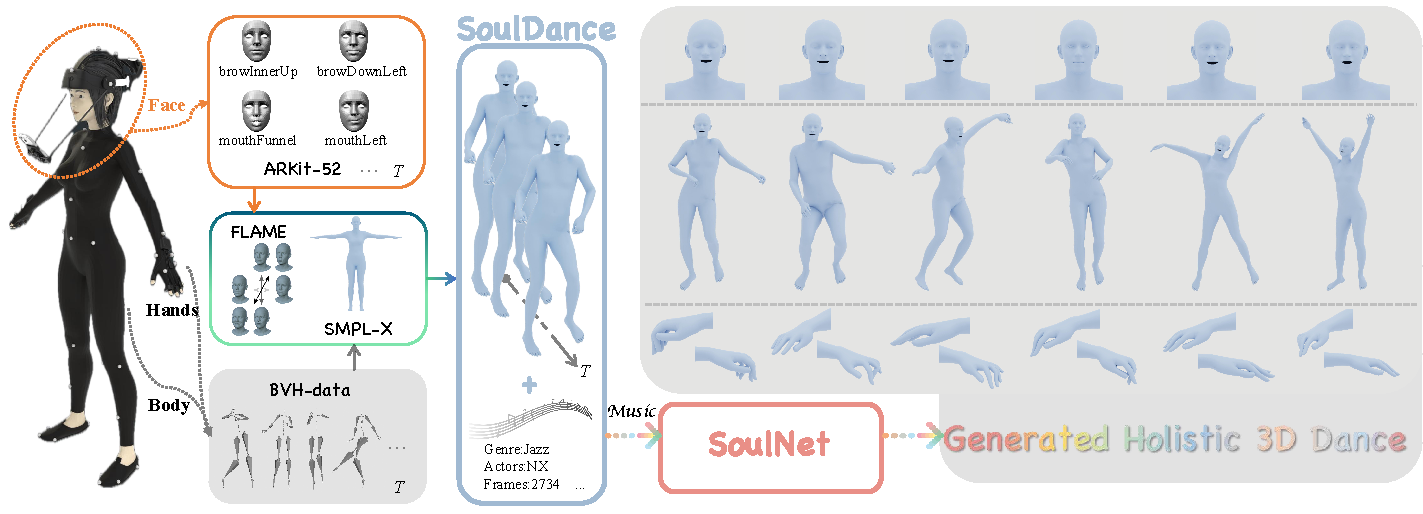
\includegraphics[width=1.0\linewidth]{figures/SoulDance/teaser.pdf}
  \caption{全身舞蹈动作数据集制作与生成流程图}
  \label{fig:souldance_teaser}
\end{figure}

\section{研究思路和框架}
大多数舞蹈数据集的采集依赖姿态估计算法~\cite{sun2022dancetrack, fang2017rmpe}，从视频中提取舞蹈动作~\cite{li2021ai, li2022danceformer, le2023music}。然而，此类处理流程通常会产生质量较低的数据，因为仅依赖视频来源难以准确获取精细的肢体动作和面部表情。所以本文首先提出了一个高表现力的全身舞蹈动作数据集SoulDance，它是首个引入面部表情的高质量3D舞蹈捕捉数据集，包括音乐与舞蹈数据对。

接下来，如图~\ref{fig:souldance_teaser}所示，利用SoulDance数据集，本章提出了舞蹈生成架构SoulNet用于生成音乐对齐的协调的全身舞蹈动作。具体而言，在给定一段音乐 $C$，生成高质量且与音乐高度匹配的整体三维舞蹈动作序列 $\tilde m_{1:N}$，其中每一帧 $\tilde m_i \in \mathbb{R}^D$，$D$ 表示姿态特征的维度，序列长度 $N$ 则由音乐 $C$ 的持续时间决定。

同时，通过引入预训练的音乐-动作检索模型（Music-Motion Retrieval, MMR）作为对齐先验，用于提升生成的舞蹈动作序列与音乐之间的一致性。此外，MMR 还为舞蹈动作空间提供了额外约束，从而降低SoulNet生成网络的训练难度，并提升最终生成舞蹈的质量。

\subsection{基于光学动捕的全身舞蹈动作数据集制作}
大多数现有的舞蹈动作数据集普遍缺乏手部动作细节，它们几乎完全忽略了面部表情，因而难以支持整体的舞蹈演绎呈现。在表~\ref{tab:data_compare} 中“Pos”与“Rot”分别表示三维位置与旋转信息；“\underline{\textit{52}}”指代与 ARKit~\cite{baruch2021arkitscenes}相关的52个面部表情参数。本章构建高质量音乐配对整体舞蹈数据集 SoulDance，包含 12.5 小时成对音乐与舞蹈数据，采用专业动作捕捉系统采集：系统配置 15 台光学摄像机、身体动作捕捉服、数据手套以及面部表情跟踪系统。与现有数据集相比，SoulDance 在同一时间轴下同时提供身体动作、手部姿态与面部表情信息，覆盖 284 段音乐片段、共 15 种音乐风格，表演者均为专业舞者。数据以多种表示形式发布，包括骨架层级 BVH 文件、SMPL-X~\cite{SMPL-X:2019}人体模型与 FLAME~\cite{FLAME:SiggraphAsia2017}面部参数，从而为整体舞蹈生成与分析研究提供高质量、丰富多样的数据基础。

\begin{table*}[ht]\footnotesize
    % \setlength\tabcolsep{3pt}
    \centering
    \caption{三维数字人舞蹈动作数据集对比}
    \resizebox{\textwidth}{!}{
        \begin{tabular}{lccccccccccc}
            \toprule [1pt] \noalign{\smallskip}
            数据集 &  Pos/Rot & 关节点数 & 手 & 脸 & 题材 & 动捕& 单人舞   & 多人舞 & SMPL & \makecell[c]{总计小时} & \makecell[c]{平均时长（秒）}\\
            \hline\noalign{\smallskip}\noalign{\smallskip}
            PMSD~\cite{valle2021transflower} & \Checkmark/\XSolidBrush & 52 & \XSolidBrush & \XSolidBrush &14 & \Checkmark & \Checkmark & \XSolidBrush & \XSolidBrush  & 3.84 & -\\
            Dance w/Melody~\cite{tang2018dance} & \Checkmark/\XSolidBrush & 21 & \XSolidBrush & \XSolidBrush & 4 & \Checkmark & \Checkmark & \XSolidBrush & \XSolidBrush & 1.6 & 92.5\\
            Music2Dance~\cite{zhuang2022music2dance} & \Checkmark/\XSolidBrush & 55 & \Checkmark & \XSolidBrush & 2 & \Checkmark & \Checkmark & \XSolidBrush & \XSolidBrush & 0.96 & -\\
            AIOZ-GDANCE~\cite{le2023music}& \Checkmark/\Checkmark & 24 & \XSolidBrush & \XSolidBrush & 7 & \XSolidBrush & \XSolidBrush & \Checkmark & \Checkmark & \textbf{16.7} & 73.8\\
            PhantomDance~\cite{li2022danceformer} & \Checkmark/\XSolidBrush & 24 & \XSolidBrush & \XSolidBrush & 13 & \XSolidBrush & \Checkmark & \XSolidBrush & \XSolidBrush &  9.6 & 133.3\\
            AIST++~\cite{li2021ai} & \Checkmark/\Checkmark & 24 & \XSolidBrush & \XSolidBrush & 10 & \XSolidBrush & \Checkmark & \XSolidBrush & \Checkmark & 5.2 & 13.3\\
            MMD~\cite{chen2021choreomaster} & \Checkmark/\Checkmark & 52 & \Checkmark & \XSolidBrush & 4  & \Checkmark & \Checkmark & \XSolidBrush & \XSolidBrush &  9.9 & -\\
            FineDance~\cite{li2023finedance}  &  \Checkmark/\Checkmark & 52 & \Checkmark & \XSolidBrush & \textbf{22} & \Checkmark & \Checkmark & \XSolidBrush & \Checkmark & 14.6 & 152.3\\
    
            \midrule [0.5pt]
            \textbf{SoulDance (Ours)} &  \Checkmark/\Checkmark & \textbf{55+\underline{\textit{52}}} & \Checkmark & \Checkmark & 15  & \Checkmark & \Checkmark & \Checkmark & \Checkmark & 12.5 & \textbf{158.5}\\
            % \noalign{\smallskip}
            \bottomrule [1pt] 
        \end{tabular}
    }
    % \vspace{0.1mm}
    \label{tab:data_compare}   
    % \vspace{-1em}
\end{table*}



% \begin{table*}[ht]
%     \setlength\tabcolsep{3pt}
%     \centering
%     \resizebox{\textwidth}{!}{
%         \begin{tabular}{lccccccccccc}
%             \toprule [1pt] \noalign{\smallskip}
%             Dataset &  Pos/Rot &  \makecell[c]{Joints\\num} & Hand & Face & Genres & Mocap& \makecell[c]{Single\\Dance}   & \makecell[c]{Group\\Dance} & SMPL & \makecell[c]{Total\\hours} & \makecell[c]{avg Sec\\per Seq}\\
%             \hline\noalign{\smallskip}\noalign{\smallskip}
%             PMSD~\cite{valle2021transflower} & \Checkmark/\XSolidBrush & 52 & \XSolidBrush & \XSolidBrush &14 & \Checkmark & \Checkmark & \XSolidBrush & \XSolidBrush  & 3.84 & -\\
%             Dance w/Melody~\cite{tang2018dance} & \Checkmark/\XSolidBrush & 21 & \XSolidBrush & \XSolidBrush & 4 & \Checkmark & \Checkmark & \XSolidBrush & \XSolidBrush & 1.6 & 92.5\\
%             Music2Dance~\cite{zhuang2022music2dance} & \Checkmark/\XSolidBrush & 55 & \Checkmark & \XSolidBrush & 2 & \Checkmark & \Checkmark & \XSolidBrush & \XSolidBrush & 0.96 & -\\
%             AIOZ-GDANCE~\cite{le2023music}& \Checkmark/\Checkmark & 24 & \XSolidBrush & \XSolidBrush & 7 & \XSolidBrush & \XSolidBrush & \Checkmark & \Checkmark & \textbf{16.7} & 73.8\\
%             PhantomDance~\cite{li2022danceformer} & \Checkmark/\XSolidBrush & 24 & \XSolidBrush & \XSolidBrush & 13 & \XSolidBrush & \Checkmark & \XSolidBrush & \XSolidBrush &  9.6 & 133.3\\
%             AIST++~\cite{li2021ai} & \Checkmark/\Checkmark & 24 & \XSolidBrush & \XSolidBrush & 10 & \XSolidBrush & \Checkmark & \XSolidBrush & \Checkmark & 5.2 & 13.3\\
%             MMD~\cite{chen2021choreomaster} & \Checkmark/\Checkmark & 52 & \Checkmark & \XSolidBrush & 4  & \Checkmark & \Checkmark & \XSolidBrush & \XSolidBrush &  9.9 & -\\
%             FineDance~\cite{li2023finedance}  &  \Checkmark/\Checkmark & 52 & \Checkmark & \XSolidBrush & \textbf{22} & \Checkmark & \Checkmark & \XSolidBrush & \Checkmark & 14.6 & 152.3\\
    
%             \midrule [0.5pt]
%             \textbf{SoulDance (Ours)} &  \Checkmark/\Checkmark & \textbf{55+\underline{\textit{52}}} & \Checkmark & \Checkmark & 15  & \Checkmark & \Checkmark & \Checkmark & \Checkmark & 12.5 & \textbf{158.5}\\
%             % \noalign{\smallskip}
%             \bottomrule [1pt] 
%         \end{tabular}
%     }
%     \vspace{0.1mm}
%     \caption{\textbf{Comparisons of 3D Dance Datasets}. ``Po" and ``Rot" represent 3D position and rotation information, respectively. ``\underline{\textit{52}}" refers to the parameters associated with ARKit blendshapes. ``avg Sec per Seq" indicates the average duration in seconds for each sequence.}
%     \label{tab:data_compare}   
%     \vspace{-1em}
% \end{table*}


\subsubsection{全身动作捕捉系统}
\label{motion_captrue}
为了获取高质量且精确的舞蹈动作数据，本章构建了一个全面的动作捕捉系统，如图~\ref{fig:souldance_teaser} 所示。该系统主要由两个部分组成。首先，采用基于标记点的专业动作捕捉系统~\cite{chingmu}对身体与手部动作进行采集，并将数据以 BVH 格式存储。其次，通过搭建一个稳定的面部表情捕捉系统，使用 iPhone 12 搭配头戴式支架（图~\ref{fig:souldance_teaser} 中的虚线椭圆所示），利用 ARKit 技术~\cite{baruch2021arkitscenes}记录包含 52 个参数的面部 blendshape 数据。整个采集过程在一个面积为 140 平方米的动作捕捉影棚中进行，共使用 15 台摄像机对舞蹈动作进行记录。舞蹈由专业编舞师根据音乐进行编排，表演者先在常规舞蹈教室中排练，待动作熟练后再进入专业捕捉棚，穿戴动作捕捉服装进行正式录制。采集过程中使用 CMAvatar 软件~\cite{chingmu}，录制帧率为 60 FPS。

% \begin{figure}[b]
%   \centering
%   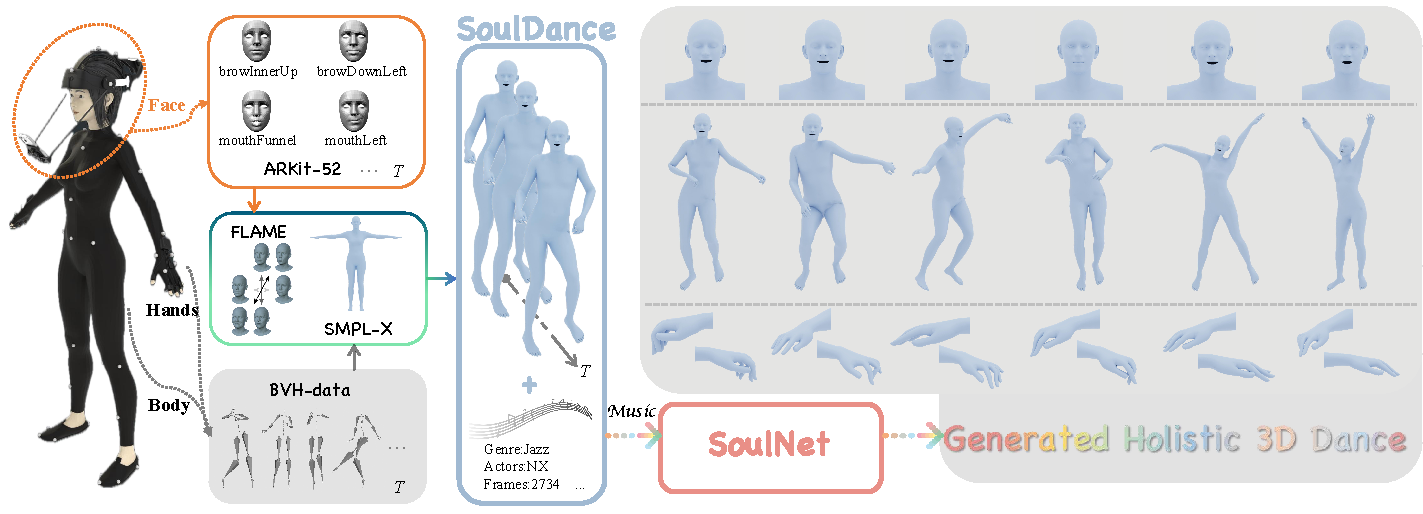
\includegraphics[width=0.8\linewidth]{figures/SoulDance/teaser.pdf}
%   \caption{数据集处理流程包含面部表情和身体-手部的动作捕捉}
%   \label{fig:souldance_teaser}
% \end{figure}

通过邀请五位专业舞者参与动捕录制，以确保舞蹈动作具备高度的专业性。在整个录制过程中，执行导演全程监督舞蹈质量及其与音乐的同步情况，同时配备技术工程师随时调整并修正录制中可能出现的不同步问题。通过这一严谨的流程，确保了高质量、精确的整体舞蹈动作数据得以采集。数据采集完成后，身体与手部的原始动作数据将经过处理并重定向到 SMPL-X 模型~\cite{SMPL-X:2019}。同时，面部的原始 ARKit 数据也被转换为与 SMPL-X 兼容的 FLAME~\cite{FLAME:SiggraphAsia2017} 参数。
% 相关细节见附录~\ref{supl:flame}。


\subsubsection{动作姿态精修}
\label{assumptions}
现有的大多数舞蹈数据集主要聚焦于身体动作，通常使用 SMPL 模型中的 24 个身体关节~\cite{SMPL2015}。相比之下，本文所提出的数据集关注更为细致的整体舞蹈动作，采用了 SMPL-X 模型~\cite{pavlakos2019expressive}，该模型包含 22 个身体关节、30 个手部关节，并与用于面部表情建模的 FLAME 参数~\cite{li2017learning} 兼容。
如图~\ref{fig:souldance_teaser} 所示，当获取到身体动作与手势的 BVH 数据后，本文使用 MotionBuilder~\cite{motionbuilder} 和 Unreal Engine (UE5)~\cite{unrealengine5} 将动作重定向至 SMPL-X 格式。在整个重定向过程中，通过在 UE5 中构建了一整套工作流程，包括 T 形姿势调整、骨骼长度校准以及关节名称映射，以确保动作的精准对齐。在必要情况下，我们的工程师团队还会对部分不符合物理规律的关节动作进行手动修正，从而进一步提升重定向动作的真实性。


\subsection{基于分层残差向量量化的动作编码}
\label{subsec:hrvq}

以往的研究~\cite{siyao2022bailando, guo2022tm2t, jiang2023motiongpt}利用 VQ-VAE 将连续舞蹈序列 $m_{1:N} \in \mathbb{R}^{N \times D}$ 量化为离散的动作 token 序列 $z_{1:N} \in \mathbb{R}^{n \times d}$，其中下采样比为 $n/N$，潜在维度为 $d$，并通过无监督方式构建可复用的码本 $\mathcal{C} = \{c_k\}_{k=1}^{K} \subset \mathbb{R}^{d}$。这一过程可表示如下：
\begin{equation}
\begin{aligned}
    \hat{m}_{1:N} = \mathcal{D}(VQ(\mathcal{E}(m_{1:N}))),
\end{aligned}
\label{eq:hrvq_rep}
\end{equation}
其中，$\mathcal{E}$ 表示将原始动作序列编码为潜在表示的编码器，$VQ(\cdot)$ 为向量量化操作，$\mathcal{D}$ 为解码器，用于将量化后的编码重新映射回动作序列 $\hat{m}_{1:N}$。然而，$VQ(\cdot)$ 操作不可避免地引入信息丢失，从而限制了重建质量。近期研究引入了残差向量量化（Residual Vector Quantization, RVQ）~\cite{zeghidour2021soundstream, yao2024moconvq, guo2024momask}，通过对前一层的残差误差进行迭代量化，有效减少量化误差。然而，RVQ 虽能降低误差，但仍难以捕捉身体、手部与面部之间的关联关系。

\begin{figure}[b]
  \centering
  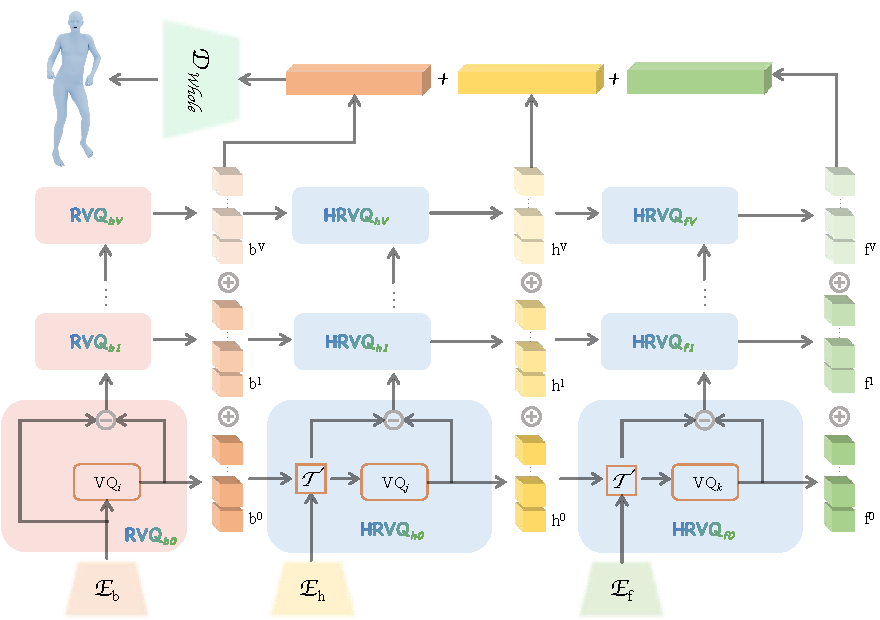
\includegraphics[width=0.8\linewidth]{figures/hrvq.pdf}
  \caption{分层残差向量量化模块}
  \label{fig:hrvq}
\end{figure}

为了利用 RVQ 的多层编码能力以建模复杂且完整的舞蹈动作，我们提出了分层残差向量量化（Hierarchical Residual Vector Quantization, HRVQ）方法。该方法构建了一个“身体–手部–面部”的多层链式结构，用于学习身体、手部与面部之间的依赖关系，如图~\ref{fig:hrvq}所示。具体而言，本文首先将整体舞蹈序列 $m_{1:N}$ 分解为三部分：身体动作 $m_{1:N}^b$、手部动作 $m_{1:N}^h$ 和面部动作 $m_{1:N}^f$。这三部分分别输入各自的编码器 $\mathcal{E}$，得到初始量化向量 $b^0$、$h^0$ 和 $f^0$。随后，对身体部分的残差 $r_b^v$ 进行迭代量化，得到每一层 $v = 0, \dots, V$ 的量化向量 $b^v$，其中 $V$ 为总层数，$b^0$ 是初始主向量，后续的 $b^{1:V}$ 表示残差的逐层逼近。该迭代结构使得多层次的信息能够被逐步编码，从而实现精细表示。接着，通过引入一个转换过程 $\mathcal{T}$，用于将手部残差 $r_h^v$ 与 $b^v$ 结合后进行量化，得到 $h^v$。面部部分采用相同方式，结合 $h^v$ 得到 $f^v$。其形式如下：
\begin{equation}
\left \{
\begin{aligned}
    & b^v=VQ_b(r^v_b) \\
    & h^v=VQ_h(\mathcal{T}(r^v_h, b^v)) \\
    & f^v=VQ_f(\mathcal{T}(r^v_f, h^v)) ,\\
\end{aligned}
\right.
\label{eq:hrvq_z}
\end{equation}
其中 $VQ_b$、$VQ_h$、$VQ_f$ 分别为身体、手部和面部的量化函数。因此，每层的残差计算如下：
\begin{equation}
\left \{
\begin{aligned}
     & r^0_b=\mathcal{E}_b(m_{1:N}^b), \quad r^{v+1}_b = r^v_b - b^v \\
    & r^0_h=\mathcal{T}(\mathcal{E}_h(m_{1:N}^h), b^0), \quad r^{v+1}_h = r^v_h - h^v \\
    & r^0_f=\mathcal{T}(\mathcal{E}_f(m_{1:N}^f), h^0), \quad r^{v+1}_f = r^v_f - f^v, \\
\end{aligned}
\right.
\label{eq:hrvq}
\end{equation}
其中 $\mathcal{E}_b$、$\mathcal{E}_h$、$\mathcal{E}_f$ 分别表示身体、手部和面部的编码器。应用 HRVQ 后，最终的舞蹈重建可表示为：
\begin{equation}
\begin{aligned}
    \hat{m}_{1:N} = \mathcal{D}_{\text{whole}}\left(\text{concat}\left(\sum_{v=0}^{V} b^v, \sum_{v=0}^{V} h^v, \sum_{v=0}^{V} f^v\right)\right),
\end{aligned}
\label{eq:hrvq_concat}
\end{equation}
其中 $\mathcal{D}_{\text{whole}}$ 为整体解码器，用于将重建后的身体、手部和面部动作融合后还原为最终的动作序列 $\hat{m}_{1:N}$。最后，本文通过结合重建误差与各层量化嵌入误差来优化分层残差 VQ-VAE，其训练损失为：
\begin{equation}
\begin{aligned}
    \mathcal{L}_{hrvq} = & \left \| m - \hat{m} \right \|_1 + \alpha \sum_{v=1}^{V}\left \| r^v_b - sg[b^v] \right \|_2 \\
& + \beta \sum_{v=1}^{V}\left \| r^v_h - sg[h^v] \right \|_2 + \gamma \sum_{v=1}^{V}\left \| r^v_f - sg[f^v] \right \|_2 ,
\end{aligned}
\label{eq:hrvq_loss}
\end{equation}
其中 $sg[\cdot]$ 表示停止梯度（stop-gradient）操作，$\alpha$、$\beta$、$\gamma$ 为各部位嵌入损失的加权系数。

通过引入分层残差向量量化编码对空间结构化的舞蹈动作序列进行编码和离散化，将其映射为多层次的码本索引。从而有效压缩了舞蹈动作空间，并捕捉了身体、手部和面部之间的先验关联信息。

\subsection{音乐对齐的舞蹈动作生成}
\label{subsec:magm}
在经过 HRVQ 量化之后，身体、手部与面部的动作 token 被拼接形成统一的整体舞蹈表示 $T_v = \text{concat}(b^v, h^v, f^v)$，其中 $v=0, \dots, V$。为了从该离散 token 序列中生成具有多样性且协调一致的整体三维舞蹈动作，需满足以下两个关键要求：（1）模型能够有效建模 token 之间的关系，保留其细节与层次结构；（2）所生成的 token 序列需与输入音乐高度对齐，以确保动作在节奏与风格上与音乐一致。

为解决上述问题，本文提出了音乐对齐生成模型，该模型旨在基于给定音乐 $C$ 条件下生成整体舞蹈动作。如图~\ref{fig:gpt} 所示，左侧为音乐对齐生成模型（Music-Aligned Generative Model, MAGM）的训练与推理流程，包含两个阶段：其一是通过 Transformer 层生成基础层的初始动作 token；其二是通过 $V-1$ 层残差量化网络逐步细化动作。右侧展示了音乐-动作检索模块（Music-Motion Retrieval, MMR）在预训练阶段中实现动作与音乐对齐的流程。完成预训练后，MMR 通过损失项 $\mathcal{L}_{\text{Align-body}}$ 与 $\mathcal{L}_{\text{Align-whole}}$ 对 MAGM 的训练过程进行监督，从而确保所生成舞蹈动作与音乐在语义与节奏上的有效对齐。
本文使用预训练的 MMR 提取音乐特征，并将其附加至初始 token 序列 $T_0$，随后对该序列施加随机掩码与位置编码，通过 Transformer 层 $\theta$ 对被掩码部分进行预测，得到重构的 $\hat{T}_0$。其优化目标为：
\begin{equation}
\begin{aligned}
    \mathcal{L}_{\text{mask}} = \sum_{t_i \in \text{mask}} -\log_{\theta} (T_0 | T_0^m, C) + \lambda_b \mathcal{L}_{\text{Align-body}},
\end{aligned}
\label{eq:mask_loss}
\end{equation}
其中 $T_0 = \{ t_i \}_{i=1}^n$ 表示初始的离散舞蹈 token 序列，$T_0^m$ 表示被随机掩码的版本。接下来，在给定音乐 $C$ 与 $T_0$ 的条件下，使用 $V-1$ 层残差网络 $\phi$ 递归预测高层残差 token $T_{1:V}$，其训练损失定义为：
\begin{equation}
\begin{aligned}
    \mathcal{L}_{\text{res}} = \sum_{i=1}^{V} -\log_{\phi} (T_{i:V} | T_0, C) + 
\lambda_w \mathcal{L}_{\text{Align-whole}},
\end{aligned}
\label{eq:res_loss}
\end{equation}
其中超参数 $\lambda_b$ 与 $\lambda_w$ 均设置为 0.5，用于平衡动作重建与音乐对齐的权重。$\mathcal{L}_{\text{Align-body}}$ 与 $\mathcal{L}_{\text{Align-whole}}$ 的对齐监督信号均来自于预训练的 MMR 模块。




\begin{figure}[h]
	\centering
	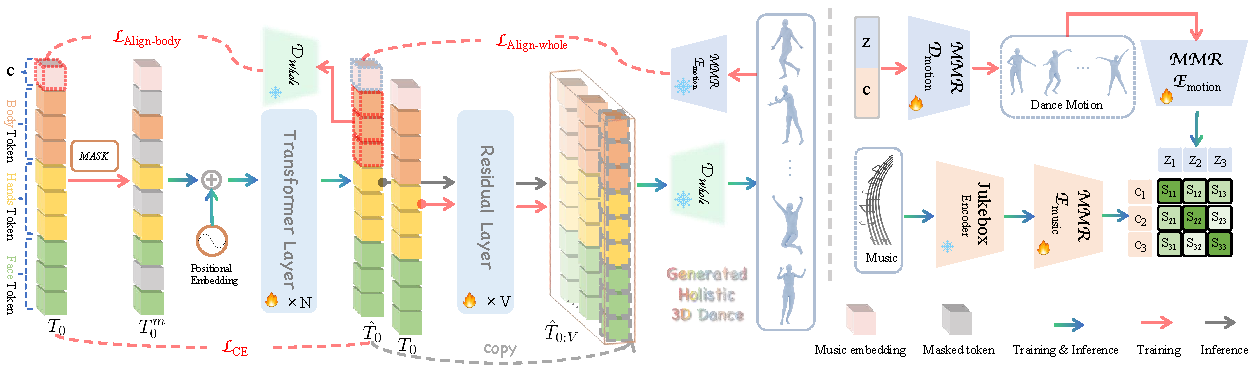
\includegraphics[width=\linewidth]{figures/SoulNet.pdf}
	\caption{SoulNet 框架概览}
	\label{fig:gpt}
	\vspace{0.5em}
\end{figure}

在音乐条件下实现精确的舞蹈-音乐对齐，一直是生成式舞蹈建模中的核心挑战。尽管在跨模态生成任务中（如文本-图像生成）已经取得了显著成果，例如通过 CLIP~\cite{radford2021learning} 建立良好的跨模态嵌入空间~\cite{rombach2022high, saharia2022photorealistic}，但在音乐-舞蹈生成领域，这一问题仍相对较少探索。现有的方法大多使用 Librosa~\cite{jin2017towards} 提取低层音频特征，或使用预训练音乐编码器如 Jukebox~\cite{dhariwal2020jukebox}，并将提取结果直接输入运动生成器。然而，这种直接映射方式忽略了音频与动作之间的模态差异，容易导致生成结果在时间和情感上难以与音乐保持同步。为解决上述模态鸿沟问题，本文提出了 音乐-动作检索模块（MMR），这是一个专为舞蹈-音乐对齐设计的跨模态建模框架。如图~\ref{fig:gpt}（右）所示，MMR 模块包含以下三个核心组成部分：

1. 动作编码（Motion Encoding）：  
   将输入的舞蹈动作序列 $M \in \mathbb{R}^{T \times D_m}$ 输入至时间编码器 $\mathcal{E}_{\text{motion}}$，通过可学习的下采样操作将其压缩为潜在表示 $\mathbf{z} = \{z_i\}_{i=1}^d$。

2. 音乐编码（Music Encoding）：  
   对原始音频输入 $C$ 先使用预训练的 Jukebox 编码器~\cite{dhariwal2020jukebox} 提取高层语义特征，再通过专门设计的音乐编码器 $\mathcal{E}_{\text{music}}$ 映射至与动作对齐的嵌入空间，得到音乐潜在表示 $\mathbf{c} = \{m_i\}_{i=1}^d$。

3. 跨模态融合（Cross-Modal Fusion）：  
   将动作嵌入 $\mathbf{z}$ 与音乐嵌入 $\mathbf{c}$ 进行拼接后，输入至基于 Transformer 的动作解码器 $\mathcal{D}_{\text{motion}}$，以生成语义一致且节奏协调的舞蹈动作序列。

本文的 MMR 模型在架构上扩展自 TEMOS 框架~\cite{petrovich2022temos}，针对舞蹈与音乐的模态特性做了定制化调整。其优化目标包括两个部分：（1）重建损失（Reconstruction Loss），用于保证生成动作的还原度；（2）对比学习损失（Contrastive Loss），采用 InfoNCE 损失~\cite{oord2018representation} 最大化正样本（配对音乐-动作）之间的互信息，同时降低负样本之间的相似性，从而增强跨模态对齐能力。

\section{实验设计与结果分析}

\subsection{实验配置}
对于 HRVQ，我们在编码器与解码器中均采用残差块结构，下采样倍率为 4。每个向量量化器由 6 层组成，且每一层的码本包含 512 维的码向量。特征变换过程采用一个 MLP 与一维卷积（1D convolution）实现。量化 dropout 比例 $q$ 设为 0.2。对于 MAGM，我们使用 6 层 Transformer 与 6 层残差 Transformer，注意力头数为 8，潜变量维度为 512。所有模型训练均采用线性 warm-up 策略：学习率在 2000 次迭代后升至 $2 \times 10^{-4}$。训练 HRVQ 的 batch size 设为 256，训练 MAGM 的 batch size 设为 64。在推理阶段，我们采用 classifier-free guidance（CFG），其 guidance scale 分别设为 4 和 5。在训练 MMR 模块时，我们使用 AdamW 优化器，学习率设为 $1 \times 10^{-4}$，batch size 设为 32。嵌入向量的潜在维度设置为 $d = 256$。温度系数 $\tau$ 设为 0.1，InfoNCE 损失的权重设为 0.1。用于过滤负样本的阈值设为 0.8。所有实验均在 4 张 NVIDIA V100 GPU 上完成，整个流程在三天内完成。

本文将所提出的方法与多个当前最先进的舞蹈生成方法进行了比较。FACT~\cite{li2021ai} 是一种自回归的舞蹈生成方法，与 AIST++ 数据集一同提出。Bailando~\cite{siyao2022bailando} 是一种基于 Transformer 的舞蹈生成方法，首次引入了 VQ-VAE 以实现舞蹈动作的离散建模。EDGE~\cite{tseng2023edge} 是一种基于扩散模型的舞蹈生成算法，在仅生成身体动作的任务中达到了较高的动作质量。FineNet~\cite{li2023finedance} 则是首个同时生成身体与手部动作的方法，随 FineDance 数据集一同发布。


\subsection{数据集}
AIST++ 数据集~\cite{li2021ai} 是当前三维舞蹈研究中广泛使用的基准数据集，共包含 1,408 个舞蹈片段，总时长约为 5.2 小时，均配有对应音乐。FineDance 数据集~\cite{li2023finedance} 通过光学动作捕捉系统采集，提供了总计 7.7 小时的舞蹈数据，包含约 831,600 帧。为确保实验的公平性，本文实验从 SoulDance 数据集中随机选取了 6.3 小时的数据用于实验。此外，所有舞蹈数据均采用我们统一的动作表示方式进行处理。最后，所有数据集按照 8:1:1 的比例划分为训练集、测试集与验证集。

\subsection{评价指标与量化结果分析}
\noindent\textbf{音乐动作匹配分数（MMR-Matching score, MMR-MS）}\quad  为了量化生成舞蹈与音乐之间的对齐程度，我们使用 MMR 编码器将两种模态投影到共享的潜在空间中。随后，计算其潜在表示之间的欧氏距离，作为 MMR-MS 指标：
\begin{equation}
\begin{aligned}
    \text{\textit{MMR-MS}} = \sqrt{\mu \cdot\sum_{i=1}^{d} (\mathbf{z}_i - \mathbf{m}_i)^2+\lambda \cdot \sum_{t=2}^T \left\Vert \Delta\mathbf{z}^t - \Delta\mathbf{m}^t \right\Vert_2},
\end{aligned}
\label{eq:mmr_ms}
\end{equation}
其中，第一个项衡量舞蹈与音乐在特征空间的距离，第二项则度量其在时间变化上的一致性。具体而言，$\mathbf{z} = \{z_i\}_{i=1}^d$ 与 $\mathbf{m} = \{m_i\}_{i=1}^d$ 分别表示舞蹈和音乐的潜在表示。为计算第二项，我们将舞蹈与音乐序列划分为不重叠的 1 秒段，得到长度为 $T$ 的序列集合。这些片段通过 MMR 编码器获得其潜在表示，进而计算相邻时间片之间的变化量，定义为：$\Delta\mathbf{z}^t = \mathbf{z}^t - \mathbf{z}^{t-1}$，$\Delta\mathbf{m}^t = \mathbf{m}^t - \mathbf{m}^{t-1}$，分别用于刻画舞蹈与音乐在潜在空间中的动态变化。在实际实验中，我们设置超参数 $\mu = 0.7$，$\lambda = 0.3$。
% 如表~\ref{tab:sotas_compare} 所示，实验结果表明，SoulNet 在音乐-动作对齐方面显著优于现有方法，展现出更高的跨模态一致性。

\begin{table*}
    \caption{在 SoulDance 数据集和 AIST++ 数据集上，不同方法的实验结果}
    \label{tab:sotas_compare}
    \resizebox{\linewidth}{!}{
        \begin{tabular}{lcccccccccccccc}
            \toprule [1pt]
            \multirow{2}{*}{Method}&
            \multicolumn{8}{c}{SoulDance Dataset} & \multicolumn{6}{c}{AIST++ Dataset} \\  \cmidrule(lr){2-9} \cmidrule(lr){10-15}
            \noalign{\smallskip}
            & FID $\downarrow $& FID$_h$ $\downarrow$ & Div $\uparrow$ & Div$_h$ $\uparrow $& MM $\uparrow $& MMR-MS $\downarrow$ & BAS $\uparrow $& EAS $\uparrow$ & FID $\downarrow $& Div $\uparrow$ & MM $\uparrow $&MMR-MS $\downarrow$ & BAS $\uparrow $&Run Time $\downarrow $ \\
            \noalign{\smallskip}\midrule[0.5pt]
            \noalign{\smallskip}
            Ground Truth & - & - & 1.322  &5.713 &-& 0.319 & 0.253 & -& - & 0.663 & - & 0.486 & 0.237 & -\\
            \midrule [0.5pt]
            FACT~\cite{li2021ai} & 1.008 & 0.408 & 0.646  &0.799 &0.656& 0.685 & 0.221 & 0.358 & 0.138 & 0.654 & 0.722 & 0.702 & 0.213 & 1.782\\
            Bailando~\cite{siyao2022bailando} & 1.379 & 2.244 & 1.307  &2.126 &1.117& 0.585 & 0.236 & 0.401 & 11.079 & 3.512 & \textbf{3.071} & 0.707 & 0.229 & 0.289\\
            EDGE~\cite{tseng2023edge} & 2.619 & 3.694 & 0.723  &4.025 &0.745& 0.716 & 0.241 & 0.246 & 21.370 & 1.562 & 1.397 & 0.687 & 0.233 & 1.521\\
            FineNet~\cite{li2023finedance} & 1.463 & 2.524 & 1.262  &3.448 &0.832& 0.694 & 0.213 & 0.263 & 3.127 & \textbf{3.836} & 0.885 & 0.696 & 0.223 & 1.637\\
            \midrule [0.5pt]
            \textbf{SoulNet (w/o. MMR)} & 0.048 & 1.454 & 1.303  &\textbf{4.178} &1.289& 0.418 & 0.240 & 0.435 & 0.206 & 0.698 & 0.855 & 0.714 & 0.232 & 0.086\\
            \textbf{SoulNet} & \textbf{0.029} & \textbf{0.375} & \textbf{1.312}  &3.423 &\textbf{1.310}& \textbf{0.369} & \textbf{0.244} & \textbf{0.594} & \textbf{0.081} & 1.649 & 1.359 & \textbf{0.580} & \textbf{0.242} & \textbf{0.086} \\
            \bottomrule [1pt] 
            %\noalign{\smallskip}
        \end{tabular}
        } 
\end{table*}

\noindent\textbf{情绪对齐分数（Emotion Alignment Score, EAS）}\quad  面部表情若能与音乐的情绪基调保持一致，将显著增强舞蹈的沉浸感与感染力。然而，现有方法普遍缺乏对生成面部表情与音乐情绪之间对齐程度的显式评估。为弥补这一空白，本文提出了情绪对齐得分（Emotion Alignment Score, EAS），用于量化生成的面部表情与音乐情绪之间的一致性。在情绪表示方面，我们采用基于 Ekman 情绪理论~\cite{ekman1971constants}的七类基本情绪模型，包括愤怒、厌恶、恐惧、快乐、悲伤、惊讶与中性。在表情识别方面，通过引入先进的面部表情识别算法~\cite{savchenko2023facial, xue2022vision}，对生成的面部表情进行分类预测，并将其与音乐所表达的真实情绪进行比较。最终，EAS 以预测结果与真实情绪标签之间的匹配准确率作为评估指标，其值越高表示面部表情与音乐情绪越一致。

\noindent\textbf{公共评价指标（Public Benchmarks）}\quad 本文采用以下多个通用指标对舞蹈生成性能进行全面评估：
(1) \textit{FID}：Fréchet Inception Distance（FID）广泛用于评估生成舞蹈分布与真实舞蹈分布之间的接近程度。采用 HumanML3D~\cite{guo2022generating} 中提出的方法，该方法已被广泛应用于动作生成研究中，用于衡量生成动作的质量~\cite{guo2024momask, lu2023humantomato, guo2022tm2t, li2023finedance}。
(2) \textit{Diversity}：该指标用于评估模型对不同音乐输入生成的舞蹈动作之间的特征差异。通过使用与 FID 相同的特征提取器计算生成样本之间的平均特征距离。
(3) \textit{Hand FID} 与 \textit{Hand Diversity}：针对手部动作的质量与多样性，本文提取手部动作特征，并分别计算其 FID 分数与多样性指标，以评估手部表现的真实感与变化程度。
(4) \textit{Multimodality}：本文遵循 Guo 等人~\cite{guo2022generating}的设定，计算每段音乐对应的10种编舞版本之间的平均特征距离，用以衡量模型在同一音乐下生成多样舞蹈的能力。
(5) \textit{Run Time}：评估模型在推理阶段生成相同长度舞蹈序列所需的平均运行时间，用于衡量其实用性与效率。
从定量与定性结果来看，本文提出的 SoulNet 在舞蹈生成的质量、多样性与表现力方面均显著优于现有方法。

% \begin{table}
\centering
    \resizebox{0.8\linewidth}{!}{
        \begin{tabular}{lccccc}
            \toprule [1pt]
            Dataset / Method
            & WS  & BS  & HS & ES & AS \\
            \noalign{\smallskip}\midrule[0.5pt]
            \noalign{\smallskip}
            AIST++ Dataset & 4.44 &5.22 &4.67&3.56&3.89\\
            FineDance Dataset & 6.89 & 6.57 &6.44&5.44 &6.67\\
            \textbf{SoulDance Dataset} & \textbf{8.56} & \textbf{8.67}&\textbf{8.22}&7.56 &\textbf{8.44} \\
            \midrule [0.5pt]
            FACT~\cite{li2021ai} & 5.00 & 5.11&5.22&5.33 &4.44 \\
            Bailando~\cite{siyao2022bailando}  & 4.78 & 5.22&5.11&5.11 &5.22 \\
            EDGE~\cite{tseng2023edge}  & 5.67 & 5.00&5.56&5.78 &5.33 \\
            FineNet~\cite{li2023finedance} & 6.44 & 5.89&6.11& 5.33&6.56 \\
            \textbf{SoulNet} & \underline{7.33} & \underline{8.45} & \underline{7.56} &\underline{\textbf{7.67}}&\underline{7.78} \\
            \bottomrule [1pt] 
            %\noalign{\smallskip}
        \end{tabular}}
        \caption{\textbf{Results of the User Study.} The top of the table presents user evaluation results for different datasets; The bottom presents the evaluation results for dance generation using different methods on \textit{SoulDance} dataset.}
    \label{tab:user_study} 
    \vspace{-1.5em}
\end{table}

% \noindent\textbf{用户研究指标}\quad 在用户研究中，总计共有28名评论员参与实验评估，其中包含 7 名专业舞者评论员。他们会对 22 对视频组进行了评估。对比形式如图所示，视频 A 和 B 的时长范围为 5 到 8 秒。每名评论员被要求回答一系列问题，每个问题均以 1 到 10 分进行评分。评分分别记为 Whole Score (WS)、Body Score (BS)、Hands Score (HS)、Emotion Score (ES) 和 Alignment Score (AS)，依次对应相应的问题。结果（Table~\ref{tab:user_study}）表明，我们提出的 SoulDance 数据集和 SoulNet 模型在所有评价指标上均优于现有的数据集和方法。

如表~\ref{tab:sotas_compare} 所示，本文在 SoulDance 和 AIST++ 两个数据集上对多种舞蹈生成方法进行了比较，结果表明，SoulNet 在 SoulDance 数据集上实现了当前最优的性能。然而，由于 AIST++ 数据集规模较小，SoulNet 在该数据集上的生成多样性略低于其他方法。实验结果表明，SoulNet 在音乐与动作对齐方面表现优越，显著超越现有主流方法。并且，更高的 EAS（情绪对齐得分）进一步说明本方法在面部表情与音乐情绪基调之间实现了更高程度的一致性。如图所示，定性结果也表明，SoulNet 能够生成高质量、具备多样性和整体协调性的舞蹈动作，充分展现出其在整体舞蹈生成任务中的先进性能。


% \begin{figure*}[h]
% 	\centering
%         % \begin{sub}
%         % \begin{minigage}
% 	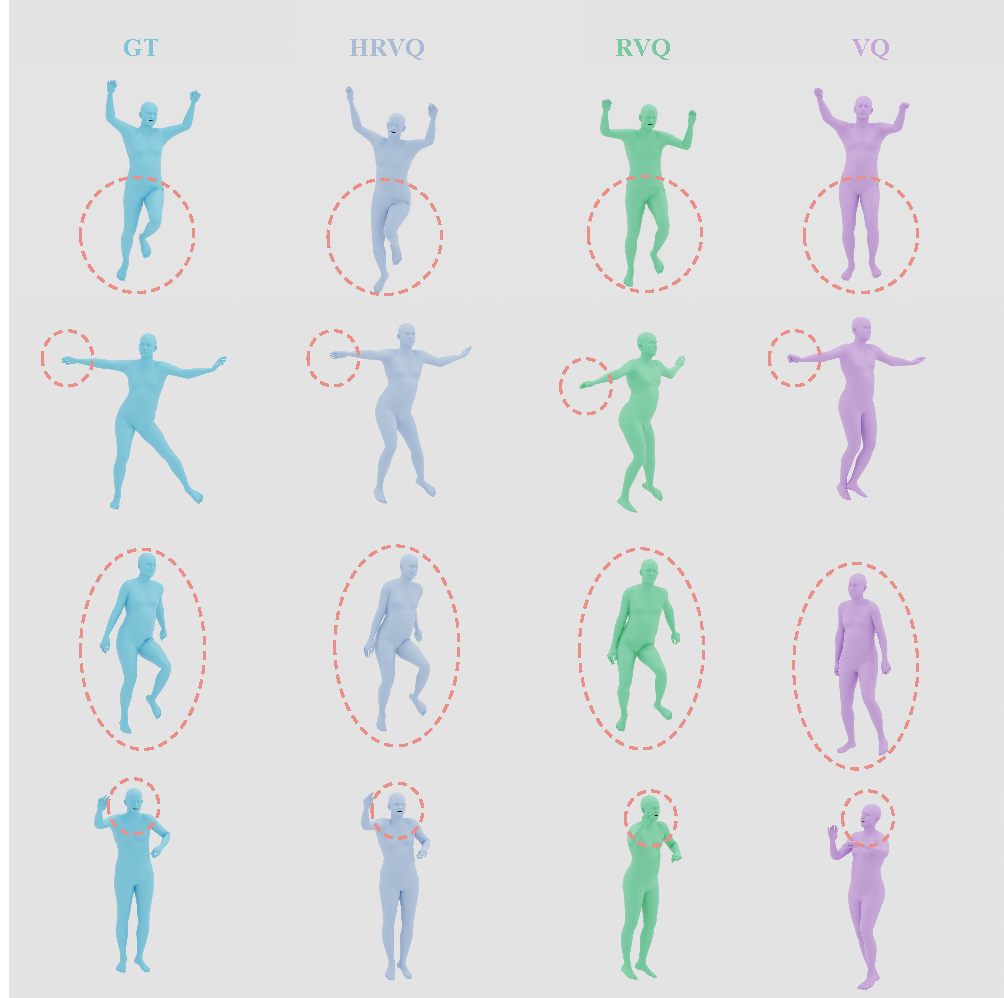
\includegraphics[width=1\linewidth]{figures/vqs_results.pdf}
%         % \vspace{-1em}
% 	\caption{数据集上的舞蹈动作重建可视化结果。}
%         \label{fig:vis_vqs}
%         % \vspace{-1.5em}
% \end{figure*}

\begin{figure}[h]
	\centering
        % \begin{sub}
        % \begin{minigage}
	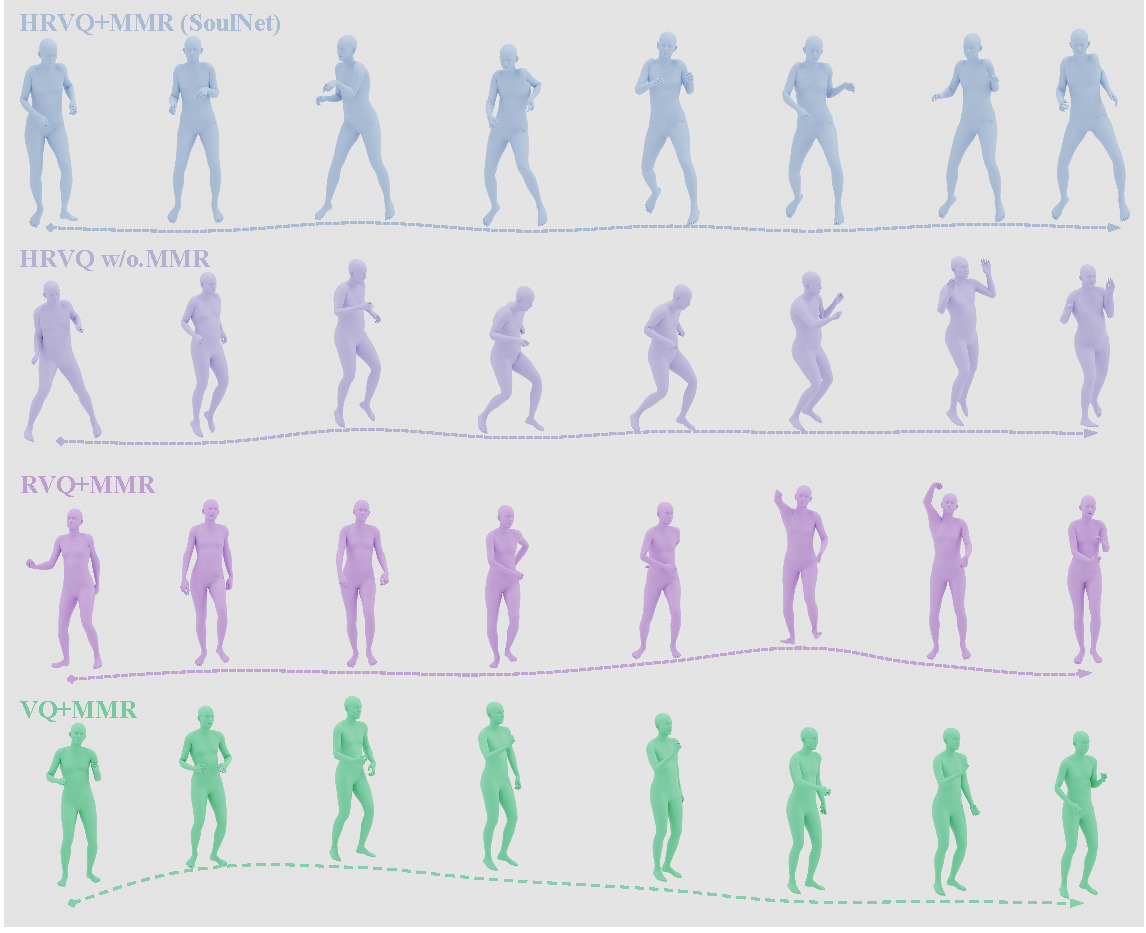
\includegraphics[width=1\linewidth]{figures/soulnet_abl.pdf}
        % \vspace{-1em}
	\caption{对比不同方法的可视化生成结果}
        \label{fig:soulnet_abl}
\end{figure}

\subsection{可视化结果分析}
除了数值上定量的比较，可视化的对比对于衡量舞蹈动作生成的好坏也尤为关键。SoulNet方法在公开舞蹈动作数据集AIST++~\cite{li2021ai}与 我们提出的SoulDance 两个数据集上都展现出卓越的效果。如图~\ref{fig:souldance_results} 所示，FACT~\cite{li2021ai} 生成的舞蹈序列在前两秒之后，身体与手部动作大多趋于静止，且完全缺失面部表情。EDGE~\cite{tseng2023edge} 能生成较为可信的身体运动，但常常无法生成细致的手部动作，并且缺乏具有表现力的面部输出。Bailando~\cite{siyao2022bailando} 能较好地捕捉身体运动与面部表情，但在转身动作中容易出现关节错位，同时手部生成也不够理想。FineNet~\cite{li2023finedance} 能生成较为令人满意的舞蹈与手部运动，但在手部精细关节刻画以及面部表情表现力方面仍存在不足。
\begin{figure}[h]
	\centering
        % \begin{sub}
        % \begin{minigage}
	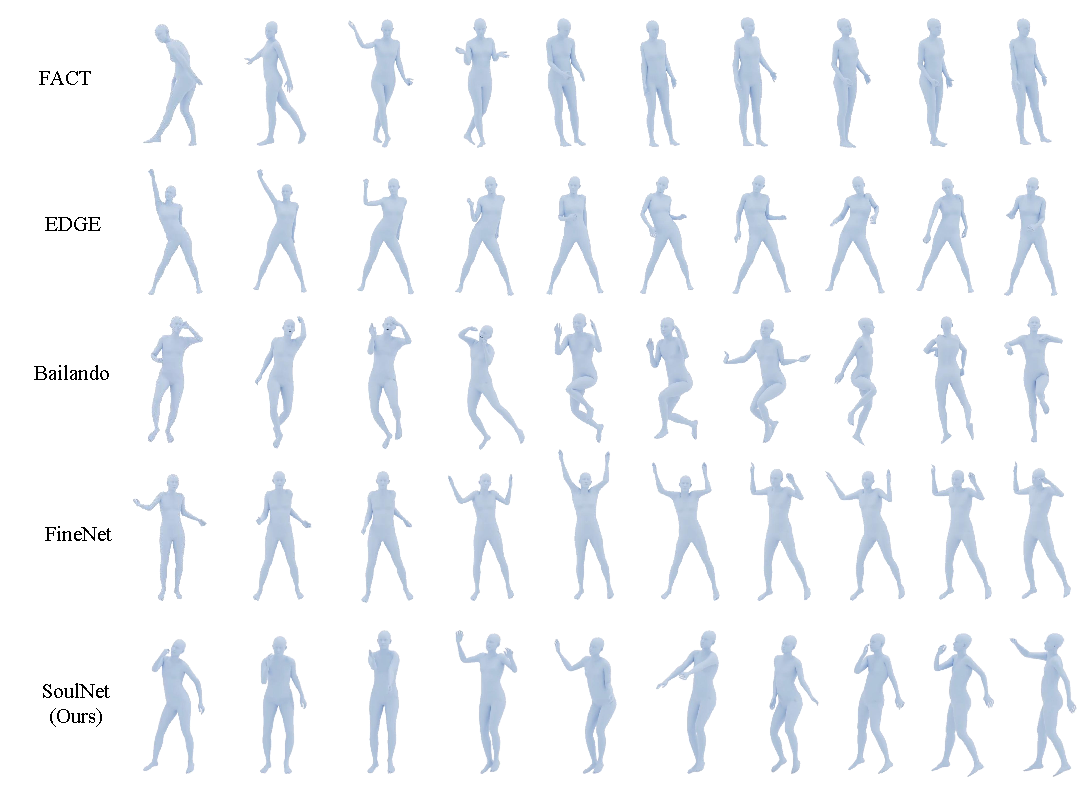
\includegraphics[width=1\linewidth]{figures/SoulDance/souldance_results.pdf}
        % \vspace{-1em}
	\caption{在同一首流行歌曲下，不同方法在SoulDance数据集上训练后生成的可视化结果}
        \label{fig:souldance_results}
        % \vspace{-1.5em}
\end{figure}

\begin{figure}[h]
	\centering
        % \begin{sub}
        % \begin{minigage}
	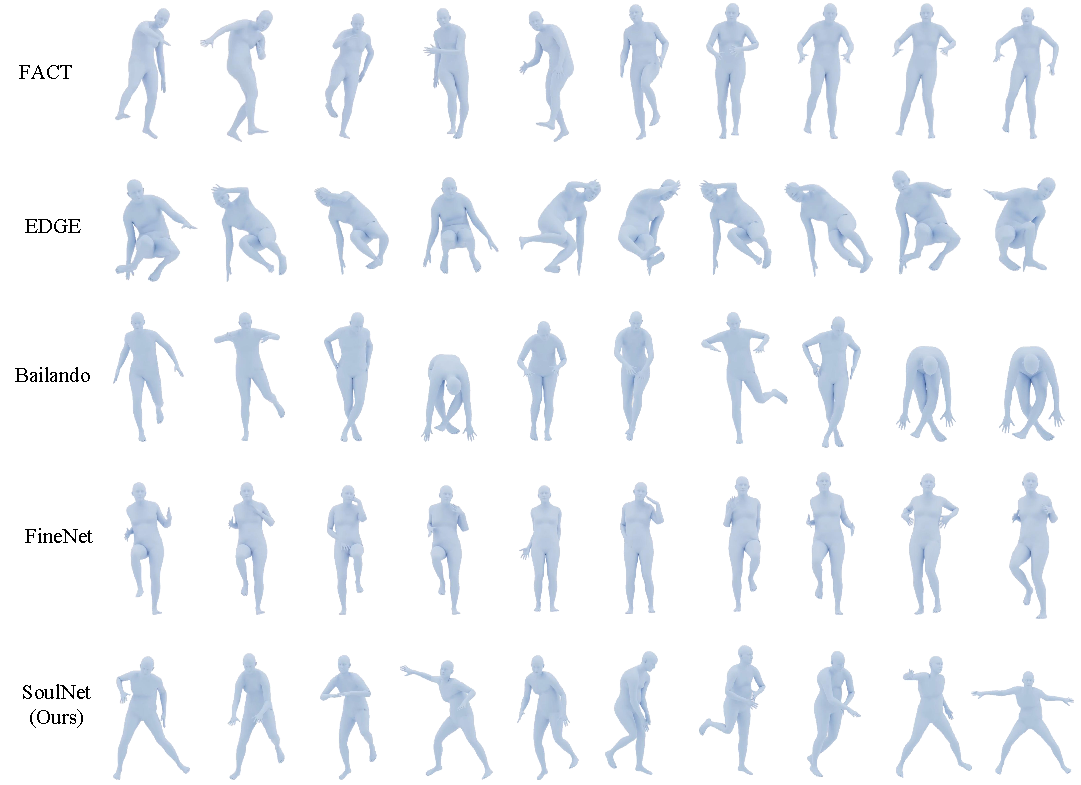
\includegraphics[width=1\linewidth]{figures/SoulDance/aistpp_results.pdf}
        % \vspace{-1em}
	\caption{在同一首摇滚歌曲下，不同方法在AIST++数据集上训练后生成的可视化结果}
        \label{fig:aistpp_results}
        % \vspace{-1.5em}
\end{figure}
相比之下，SoulNet不仅能够生成多样且富有动态变化的身体动作，还能更好地刻画复杂细致的手部与面部细节。如图~\ref{fig:aistpp_results} 所示，在 AIST++ 数据集上，SoulNet 相较于其他方法在音乐节拍对齐方面表现更优，同时生成的舞蹈序列也呈现出更高的多样性。

\subsection{消融实验}
\textbf{不同的 VQ 方法效果对比}\quad  在表~\ref{tab:vqs_compare} 中，使用 MPJPE（单位为毫米）评估不同量化方法在动作重建任务中的性能表现，以衡量三维关节位置的重建精度。同时，为评估面部动作的重建质量，本文采用 Face Vertex Error（单位为 $10^{-4}$ 毫米）作为指标，用于度量重建面部顶点与真实面部之间的平均误差。本文对多种基于向量量化（VQ）的技术进行了全面评估，以比较它们在舞蹈动作重建任务中的性能表现。
% 在图~\ref{fig:vis_vqs}中做了可视化实验，从左至右，依次展示了真实动作（GT）、HRVQ、RVQ 和 VQ 方法的重建结果。实验在相同码本大小为 512 的配置下，三种量化方法（HRVQ、RVQ 和 VQ）对同一真实舞蹈序列的重建效果对比。结果清晰地表明，HRVQ 在各个关键方面均优于其他方法，包括身体动作的重建（第1与第3行）、手部动作（第2行）以及面部表情（第4行）。
此外，图~\ref{fig:soulnet_abl} 显示，HRVQ 生成的舞蹈序列在稳定性与连贯性方面表现最优，其次为 RVQ，而 VQ 的性能最差。这些结果充分体现了 HRVQ 在捕捉细腻且富有表现力的舞蹈动作方面的优势，其重建质量显著优于 RVQ 与 VQ。
结果显示，本文提出的 HRVQ 方法在重建误差方面显著优于传统的 VQ 与 RVQ 技术，达到了当前最优水平。

\begin{table}
    % \resizebox{\linewidth}{!}{
    \caption{对比不同 VQ 方法的重建效果}
    \label{tab:vqs_compare}
    \centering
    \resizebox{0.8\linewidth}{!}{
        \begin{tabular}{lcccccccc}
            \toprule [1pt]
            \noalign{\smallskip}
            \multirow{2}{*}{Method}& \multicolumn{4}{c}{SoulDance Dataset} & \multicolumn{3}{c}{FineDance Dataset} & \multicolumn{1}{c}{AIST++ Dataset} \\  \cmidrule(lr){2-5} \cmidrule(lr){6-8} \cmidrule(lr){9-9}
            \noalign{\smallskip}
            & $all\downarrow$ & $body\downarrow$ & $hand\downarrow$ & $face\downarrow$ & $all\downarrow$ & $body\downarrow$ & $hand\downarrow$ & $body\downarrow$ \\
            \noalign{\smallskip}\midrule [0.5pt]
            \noalign{\smallskip}
            Vanilla VQ (512) & 137.130 & 97.660 & 129.518  &4.013 &	137.646	& 96.598 & 136.329 & 42.513\\
            Vanilla VQ (1024) & 136.752 & 95.809 & 128.628 & 3.739 & 136.785 & 97.328 & 135.194 & 41.369\\
            RVQ-5 & 108.983 & 71.831 & 106.836 &  2.379 & 98.399 & 59.281 & 102.706 & 24.246 \\
            HRVQ-5 (Ours) & \textbf{83.679} & \textbf{47.895} & \textbf{85.085} & \textbf{1.153} & \textbf{90.705} &\textbf{51.708} & \textbf{95.563} & \textbf{24.246} \\
            \bottomrule [1pt] 
            \noalign{\smallskip}
    \end{tabular}}
    % \vspace{1em}
\end{table}

在表~\ref{tab:abl_soulnet} 中，本文进一步对不同 VQ 方法在 SoulDance 数据集上的舞蹈动作生成性能进行了对比评估。图~\ref{fig:soulnet_abl} 中对不同方法在 SoulDance 数据集上的舞蹈生成结果进行了可视化。图中虚线表示沿重力方向的动作轨迹，轨迹波动越小，说明所生成的舞蹈动作越稳定、自然。该可视化有助于直观比较不同方法在动作连续性与身体重心控制方面的表现。定性结果也清晰地显示，HRVQ 在动作自然性与细节表现方面均优于其他方法。综上所述，HRVQ 在动作重建与舞蹈生成两个任务中均展现出稳定且领先的性能，确立了其在该领域中的先进地位。
\begin{table}
    \caption{HRVQ 和 MMR 的消融实验}
    \label{tab:abl_soulnet} 
    \centering
    \resizebox{0.6\linewidth}{!}{
        \begin{tabular}{lccccc}
            \toprule [1pt]
            Method
            & FID $\downarrow$ & Div $\uparrow$ & MM $\uparrow$ & BAS $\uparrow$ & MMR-MS $\downarrow$ \\
            \noalign{\smallskip}\midrule[0.5pt]
            \noalign{\smallskip}
            VQ-512 & 1.610 & 0.540 & 0.509  &0.237 &0.703\\
            VQ-512 + MMR & 1.552 & 0.563 & 0.576  &0.241 &0.697\\
            RVQ-512 & 0.082 & 1.308 & 1.233  &0.216 &0.571\\
            RVQ-512 + MMR & 0.067 & \textbf{1.329} & 1.250  &0.242 &0.540\\
            RVQ-1024 + MMR & 0.090 & 1.182 & 1.228  &0.234 &0.603\\
            HRVQ-512 & 0.048 & 1.303 & 1.289  &0.240 &0.418\\
            HRVQ-512 + MMR & \textbf{0.029} & 1.312 & \textbf{1.310}  &\textbf{0.244} &\textbf{0.369}\\
            \bottomrule [1pt] 
            %\noalign{\smallskip}
        \end{tabular}
        }

\end{table}

\textbf{量化层数的影响}\quad  在表~\ref{tab:diff_hrvq_v} 中，本文将残差量化层数 $V$ 从 1 增加至 7，以系统性地探讨不同层数对动作重建质量的影响。通过这一实验设置，我们能够分析在 HRVQ 框架下，量化深度与重建精度之间的关系，从而为最佳参数选择提供依据。实验分析了在 HRVQ 与 RVQ 两种方法下，不同残差量化层数 $V$ 对重建性能的影响。总体而言，增加残差量化层数有助于提升动作重建的精度，但同时也会增加 MAGM 在舞蹈 token 生成阶段的计算负担。
\begin{table}[t]
    % \resizebox{\linewidth}{!}{
    \caption{不同层的层次化残差对结果的影响}
    \label{tab:diff_hrvq_v} 
    \centering
    \resizebox{0.7\linewidth}{!}{
        \begin{tabular}{lcccccccc}
            \toprule [1pt]
            \noalign{\smallskip}
            \multirow{2}{*}{Method}& \multicolumn{4}{c}{HRVQ} & \multicolumn{4}{c}{RVQ} \\  \cmidrule(lr){2-5} \cmidrule(lr){6-9}
            \noalign{\smallskip}
            & $all\downarrow$ & $body\downarrow$ & $hand\downarrow$ & $face\downarrow$ & $all\downarrow$ & $body\downarrow$ & $hand\downarrow$ & $face\downarrow$ \\
            \noalign{\smallskip}\midrule [0.5pt]
            \noalign{\smallskip}
            V=1 & 104.859 & 67.470 & 103.092 &1.990 &126.071&86.234&120.795&3.224\\
            V=2 & 98.180 & 61.156 & 97.365 & 1.694 &121.383&81.795&116.148&2.856 \\
            V=3 & 92.777 & 55.533 & 93.776 & 1.502 &111.660&78.883&106.972&2.618 \\
            V=4 & 85.035 & 51.360 & 85.973 & 1.291 &113.503&72.570&111.069&2.475\\
            V=5 & 83.679 & 47.895 & 85.085 & 1.153 &108.983&71.831&106.836&2.379\\
            V=6 & \textbf{79.518} & 46.806 & \textbf{80.015} & 1.117 & 105.846 &65.947&105.208&2.223 \\
            V=7 & 84.080 & \textbf{46.573} & 86.218 & \textbf{1.007} & \textbf{101.209}&\textbf{63.457}&\textbf{99.794}&\textbf{2.098} \\
            \bottomrule [1pt] 
            \noalign{\smallskip}
    \end{tabular}}
\end{table}
如图~\ref{fig:abl_fid_mmr} 所示，当残差层数超过 5 或 6 层时，无论是在 RVQ 还是 HRVQ 中，生成质量均出现明显下降。因此，为在重建精度与生成效率之间取得平衡，SoulNet 在设计上采用了 $V=5$（即 5 层残差 VQ 层）的 HRVQ 配置，兼顾性能与效率。

\begin{figure}[h]
	\centering
        % \begin{sub}
	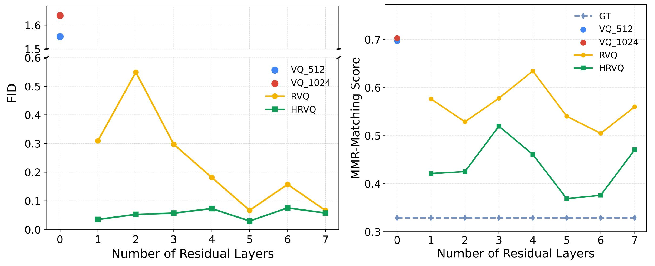
\includegraphics[width=0.8\linewidth]{figures/abl_fid_mmr.pdf}
        % \vspace{-1em}
	\caption{不同量化方法在不同残差层数配置下的性能对比}
        \label{fig:abl_fid_mmr}
\end{figure}

\textbf{音乐对齐策略效果}\quad  为验证所提出音乐对齐策略的有效性，本文对比了引入与不引入 MMR 模块条件下的舞蹈生成结果。 如表~\ref{tab:abl_soulnet} 所示，分别采用码本大小为 512 和 1024 进行实验，并对比在有无 MMR 监督条件下的表现差异，引入 MMR 模块不仅提升了生成舞蹈的整体质量，还显著增强了舞蹈与音乐之间的对齐效果。 同时，定性结果也进一步验证了该策略在表现力方面的提升，更多可视化示例可参见图~\ref{fig:soulnet_abl}。 这一观察结果凸显了 MMR 模块在提升音乐驱动舞蹈生成质量与同步性方面的重要作用。 此外，为进一步分析各对齐损失项的具体贡献，我们对 $\mathcal{L}_{\text{Align-body}}$ 与 $\mathcal{L}_{\text{Align-whole}}$ 进行了消融实验。 如表~\ref{tab:abl_alignloss} 所示，
本文在 SoulDance 数据集上开展实验，分别比较对齐损失项 $\mathcal{L}_{\text{Align-body}}$ 与 $\mathcal{L}_{\text{Align-whole}}$ 对舞蹈动作与音乐对齐效果的影响。 实验结果显示，两者在对齐机制中发挥互补作用：$\mathcal{L}_{\text{Align-body}}$ 更侧重于提升局部动作与音乐节奏的匹配程度，而 $\mathcal{L}_{\text{Align-whole}}$ 则有助于增强整体结构层面的同步性。 该实验验证了分层对齐策略在提升音乐驱动舞蹈生成一致性方面的重要性。$\mathcal{L}_{\text{Align-body}}$ 能有效提升局部特征的对齐效果（例如 FID 与 BAS 指标），而 $\mathcal{L}_{\text{Align-whole}}$ 则主要在整体结构对齐方面发挥作用，显著优化 MMR-MS 指标。 这表明两种对齐损失在不同粒度层面对生成结果具有互补性的提升作用。

\begin{table}[ht]
\centering
\caption{音乐对齐策略消融实验}
\label{tab:abl_alignloss} 
\resizebox{0.6\linewidth}{!}{
	\begin{tabular}{lccccccc}
	\toprule [1pt] 
	\multicolumn{2}{c}{Ablations} & \multicolumn{5}{c}{Metrics} \\ \cmidrule(lr){1-2}   \cmidrule(lr){3-7}   
        $\mathcal{L}_{\text{Align-body}}$  & $\mathcal{L}_{\text{Align-whole}}$ & FID $\downarrow$ & Div $\uparrow$ & MM $\uparrow$ & BAS $\uparrow$ & MMR-MS $\downarrow$ \\
	\noalign{\smallskip}\hline\noalign{\smallskip}
         \checkmark  & \checkmark &  \textbf{0.029} & 1.312 & 1.310  &\textbf{0.244} &\textbf{0.369}\\
         \checkmark  &   &0.031  &1.331  &1.327&0.242&0.387\\
         &  \checkmark &0.042  &\textbf{1.344} &\textbf{1.338}&0.237&0.372\\
		\bottomrule [1pt] 
               \noalign{\smallskip}
	\end{tabular}}
        % \vspace{-1em}  
\end{table}


\section{本章小结}
在本章节中提出了一个面向音乐驱动舞蹈生成任务的大规模高质量三维全身（holistic）的舞蹈动作数据集SoulDance，它能够同步捕捉身体动作、手部姿态以及面部表情。进一步地提出了 SoulNet，其利用 HRVQ 对全身舞蹈进行联合建模与高效量化。同时，使用从 MMR 中提取的音乐-舞蹈对齐先验来监督舞蹈动作生成框架，使得SoulNet能够生成与输入音乐对齐、表现力丰富的全身舞蹈序列。此外，本章还提出了两项新的评估指标用于衡量面部与身体运动与音乐之间的对齐程度。定量与定性实验结果均表明，SoulNet在生成与音乐对齐的全身舞蹈方面取得了当前最先进的性能。
